% !TeX program = pdflatex
\documentclass[11pt,a4paper,oneside]{report}             % Single-side
%\documentclass[11pt,a4paper,twoside,openright]{report}  % Duplex

\input{include/packages}



%\input{include/thesis-hu}  % Beállítások magyar nyelvű dolgozathoz
%--------------------------------------------------------------------------------------
% Elnevezések
%--------------------------------------------------------------------------------------
\newcommand{\dolgozatnyelve}{\selectlanguage{english}}

\newcommand{\bme}{Budapest University of Technology and Economics}
\newcommand{\vik}{Faculty of Electrical Engineering and Informatics}

\newcommand{\bmemit}{Department of Measurement and Information Systems}

\newcommand{\keszitette}{Author}
\newcommand{\konzulens}{Advisor}

\newcommand{\bsc}{Bachelor's Thesis}
\newcommand{\msc}{Master's Thesis}

\newcommand{\pelda}{Example}
\newcommand{\definicio}{Definition}
\newcommand{\tetel}{Theorem}

\newcommand{\bevezeto}{Introduction}
\newcommand{\koszonetnyilvanitas}{Acknowledgements}
\newcommand{\abrakjegyzeke}{List of Figures}
\newcommand{\tablazatokjegyzeke}{List of Tables}
\newcommand{\irodalomjegyzek}{Bibliography}
\newcommand{\fuggelek}{Appendix}

\newcommand{\szerzo}{\vikszerzoKeresztnev{} \vikszerzoVezeteknev}

\newcommand{\englishParagraph}{
	\setlength{\parindent}{0em} % angol nyelvű dokumentumokban jellemző
	\setlength{\parskip}{0.5em} % angol nyelvű dokumentumokban jellemző
	\nonfrenchspacing
	\renewcommand{\figureautorefname}{Figure}
	\renewcommand{\tableautorefname}{Table}
	\renewcommand{\partautorefname}{Part}
	\renewcommand{\chapterautorefname}{Chapter}
	\renewcommand{\sectionautorefname}{Section}
	\renewcommand{\subsectionautorefname}{Section}
	\renewcommand{\subsubsectionautorefname}{Section}
}


\newcommand{\hungarianParagraph}{
	\setlength{\parindent}{2em} % angol nyelvű dokumentumokban jellemző
	\setlength{\parskip}{0em}   % angol nyelvű dokumentumokban jellemző
	\frenchspacing
}

\newcommand{\defaultParagraph}{
	\englishParagraph
}

\newcommand{\ie}{i.e.\@\xspace}
\newcommand{\Ie}{I.e.\@\xspace}
\newcommand{\eg}{e.g.\@\xspace}
\newcommand{\Eg}{E.g.\@\xspace}
\newcommand{\etal}{et al.\@\xspace}
\newcommand{\etc}{etc.\@\xspace}

\bibliographystyle{plain}
 % Settings for English documents

%--------------------------------------------------------------------------------------
% Main variables


%--------------------------------------------------------------------------------------
\newcommand{\vikszerzoVezeteknev}{Kővári}
\newcommand{\vikszerzoKeresztnev}{Zsolt}
\newcommand{\vikkonzulensA}{Gábor Szárnyas} % Első konzulens neve
\newcommand{\vikkonzulensB}{Dr. István Ráth} % Második konzulens neve; hagyd üresen, ha egy konzulensed van.
\newcommand{\vikcim}{Performance Analysis of Graph Queries} % Cím
\newcommand{\viktanszek}{\bmemit} % Tanszék
\newcommand{\vikdoktipus}{} % Dokumentum típusa (diplomaterv, szakdolgozat, TDK-dolgozat, stb.)

\input{include/tdk-variables.tex}
\newcommand{\szerzoMeta}{\vikszerzoVezeteknev{} \vikszerzoKeresztnev} % egy szerző esetén
%\newcommand{\szerzoMeta}{\vikszerzoVezeteknev{} \vikszerzoKeresztnev, \tdkszerzoB} % két szerző esetén

\input{include/preamble.tex}


%--------------------------------------------------------------------------------------
% Table of contents and the main text
%--------------------------------------------------------------------------------------
\begin{document}



%~~~~~~~~~~~~~~~~~~~~~~~~~~~~~~~~~~~~~~~~~~~~~~~~~~~~~~~~~~~~~~~~~~~~~~~~~~~~~~~~~~~~~~


\pagenumbering{gobble}
\dolgozatnyelve
\englishParagraph
\singlespacing
%\include{include/project}
\onehalfspacing
\defaultParagraph



%~~~~~~~~~~~~~~~~~~~~~~~~~~~~~~~~~~~~~~~~~~~~~~~~~~~~~~~~~~~~~~~~~~~~~~~~~~~~~~~~~~~~~~
	%\include{include/titlepage}		   % Szakdolgozat/Diplomaterv címlap
	\include{include/titlepage_tdk}	% TDK címlap
	%\include{include/titlepage_otdk}   % OTDK címlap
 

% Table of Contents
%~~~~~~~~~~~~~~~~~~~~~~~~~~~~~~~~~~~~~~~~~~~~~~~~~~~~~~~~~~~~~~~~~~~~~~~~~~~~~~~~~~~~~~
	\tableofcontents\vfill


% Declaration and Abstract
%~~~~~~~~~~~~~~~~~~~~~~~~~~~~~~~~~~~~~~~~~~~~~~~~~~~~~~~~~~~~~~~~~~~~~~~~~~~~~~~~~~~~~~
	\pagenumbering{roman}
\setcounter{page}{1}

\selectlanguage{magyar}
%\hungarianParagraph

\englishParagraph
%----------------------------------------------------------------------------
% Abstract in Hungarian
%----------------------------------------------------------------------------
\chapter*{Kivonat}\addcontentsline{toc}{chapter}{Kivonat}

A gráf alapú adatmodellező, illetve adatbázis-kezelő keretrendszerek esetén kulcsfontosságú a minél nagyobb teljesítmény, illetve rövidebb válaszidő biztosítása, különösen az olyan alkalmazási területeken, ahol egyszerre több, strukturálisan összetett lekérdezést kell újra és újra kiértékelni egy folyamatosan változó (gráf)adatstruktúra felett. A modern, relációs adatmodellt elvető NoSQL technológiák terjedésével egyre nagyobb figyelmet kap az ilyen rendszerek teljesítőképessége és skálázhatósága, így az utóbbi években több olyan benchmark is megjelent, melynek fő célja az ilyen rendszerek teljesítőképességének, különösen a lekérdezések skálázhatóságának szisztematikus kiértékelése. 

A legtöbb mérési keretrendszer számításba vesz bemenet és teljesítmény leíró metrikákat, mint például a gráf csomópontjainak száma vagy a lekérdezések válaszideje, ugyanakkor nagyon nehéz az eredmények összehasonlítása, mert a méréshez használt bemenetek (gráfok, lekérdezések komplexitása, illetve a gráfon a mérés során végrehajtott változtatások jellege, összességében a \emph{terhelési profil}) igen nagy méret- és tulajdonságbeli eltéréseket mutatnak - ezekről pedig megelőző kutatási eredmények kimutatták, hogy jelentős és változó mértékben befolyásolhatják az egyes eszközök viselkedését, teljesítménykarakterisztikáját.
% Azonban, ezen keretrendszerek nem veszik figyelembe a gráf belső hálózatán végbemenő változásokat, és kizárólag egy struktúrájú gráfra koncentrálnak. 

A jelen dolgozat elsődleges célja, hogy - korábbi kutatásokat folytatva - kidolgozzon egy olyan mérési módszertant és hozzá kapcsolódó keretrendszert, amelynek segítségével a gráf alapú adatbázis-kezelő rendszerek teljesítménybeli összehasonlítása szisztematikusan és reprodukálhatóan hajtható végre. Fő eredményként a teljesítménymérés céljára különböző gráf topológiákat javasolunk, amelyek jellemzésére gráfmetrikákat definiálunk. A metrikák segítségével jellemezhető az egyes mérések nehézsége, illetve bizonyos eszközök esetén kapcsolatot is találhatunk a gráfokat jellemző metrikák és a lekérdezések futásidői között. A módszertan és a keretrendszer képességeinek bemutatására a dolgozat bemutat egy komplex esettanulmányt, mely magába foglalja számos kísérlet automatizált elvégzését és magasszintű statisztikai analízis eszközökkel támogatott kiértékelését is.

%, így metrikáink később felhasználhatóak a gráflekérdezések optimalizálása - jelenleg még nagyon kiforratlan - területén. 



\vfill
\selectlanguage{english}
\englishParagraph


%----------------------------------------------------------------------------
% Abstract in English
%----------------------------------------------------------------------------
\chapter*{Abstract}\addcontentsline{toc}{chapter}{Abstract}
Achieving high-performance query evaluation represents a crucial problem in modern graph-based database systems. The response time of the query evaluation on a graph is affected by the complexity of the particular query and the underlying network structure of the graph. 

Several state-of-the-art benchmark frameworks exist that assess the performance and correctness of query evaluations as they create real world-like workloads and define suites of systematic queries. However, these benchmark frameworks rely on only one particular type of network and they do not concentrate on a significant alteration of the underlying graph. Although most of them define metrics for characterizing the specific aspects of performance (response time, query evaluations per hour, etc.), most of them lack such comprehensive metrics for the queries and the graph.
As a consequence, they cannot determine the correlations between workload and performance.

%Due to the absence of metrics, it is difficult to give a precise characterization of the complexity for various benchmarks. Hence, it is difficult %to compare the benchmarks and the published results to each other.

In order to provide solid foundations to characterize the complexity of graph benchmarks, we elaborate a benchmark framework for graph-based database systems.

We use various graph metrics to describe the structure of the graph %create regression models to determine the relationships quantitatively.
and use a varied set of graph topologies for benchmarking. This will allow us to perform in-depth analysis on the relationships between the structure of the graph in the database and the performance of the query evaluations. These results can be used to obtain advanced heuristics for the optimization of graph query engines. While the optimization of relational databases has well-known techniques documented by a wide literature, the problem for graph query engines is yet be discussed thoroughly.




%The performance of query evaluations depends on the topology of the model, and the complexity of the particular query. Our primary goal is that --- %by defining model and query-related quantitative metrics ---  to find a considerable connection between metrics and the performance, and thus, be %able to predict the query evaluation time.

%Based on the metrics and their effect to the performance, we are able to make decisions in design to achieve on the optimal performance. %Furthermore, this knowledge can be utilized in the area of real-time query optimization engines as well.

%We investigate various NoSQL database systems via regression analysis in order to find different model-related metrics that are suited to %characterize their performance appropriately. Based on a real model, we generate graphs with various topologies and distributions to find metrics %from different aspects.

%Furthermore, we explore that whether an arbitrarily structured model's performance is predictable via our regression analysis, and also predict %which database system from our scope can be associated to the model in order to achieve an optimal performance.

%Finally, being motivated by the real-time optimization engines, we search answers whether by reducing the cost of metric calculations, an arbitrary %model's performance is still predictable.


\vfill
\dolgozatnyelve
\defaultParagraph

\newcounter{romanPage}
\setcounter{romanPage}{\value{page}}
\stepcounter{romanPage}	  %TODO Összefoglaló -- TDK és OTDK esetén nem kötelező


% The main part of the thesis
%~~~~~~~~~~~~~~~~~~~~~~~~~~~~~~~~~~~~~~~~~~~~~~~~~~~~~~~~~~~~~~~~~~~~~~~~~~~~~~~~~~~~~~
\pagenumbering{arabic}

	%\newpage
\begin{enumerate}
	\item \textbf{Introduction}
	\begin{enumerate}[label*=\arabic*.]
		\item \textbf{Problem}
		\item \textbf{Concepts}
			\item \textbf{Contributions}
			\item \textbf{Structure of the Report}
		\end{enumerate}
		\item \textbf{Background}
		\begin{enumerate}[label*=\arabic*.]
			\item \textbf{NoSQL}
			\item \textbf{RDF}
			\item \textbf{Statistics}
			\begin{enumerate}[label*=\arabic*.]
				\item \textit{Population and Sample}
				\item \textit{Distributions}
				\item \textit{Correlation}
				\item \textit{Regression}
			\end{enumerate}
			\item \textbf{Graph Theory}
			\begin{enumerate}[label*=\arabic*.]
				\item \textit{Metrics}
				\item \textit{Random-Graph}
				\item \textit{Scale-Free}
				\item \textit{Watts-Strogatz}
				\item \textit{Hierarchical}
			\end{enumerate}
		\end{enumerate}
	
	
	\item \textbf{Related Works}
	\begin{enumerate}[label*=\arabic*.]
		\item \textbf{Graph Analysis}
		\begin{enumerate}[label*=\arabic*.]
			\item \textit{Studies of Barabási and Albert}
			\item \textit{Network Robustness and Metric Correlations}
			\item \textit{Chinese Network Analysis}
			\item \textit{Conclusion}
		\end{enumerate}
		\item \textbf{NoSQL Benchmarks} or RDF / SPARQL Benchmarks
		\begin{enumerate}[label*=\arabic*.]
			\item \textit{YCSB}: maybe its not necessary
			\item \textit{Berlin}
			\item \textit{DBpedia}
			\item \textit{SP2}
			\item \textit{Conclusion}
		\end{enumerate}
	\end{enumerate}
	
	
	
	\item \textbf{Train Benchmark Framework}
	\begin{enumerate}[label*=\arabic*.]
		\item \textbf{Main Concepts}
		\item \textbf{Workflow}
		\item \textbf{The Domain}
		\item \textbf{Supported Formats}
		\item \textbf{Performance Comparison and Uniformity}
		\item \textbf{Tools}
		\item \textbf{Framework's Architecture}
	\end{enumerate}

	
	\item \textbf{Contributions}
	\begin{enumerate}[label*=\arabic*.]
		\item \textbf{Disadvantages of the Train Benchmark Domain} (necessary?)
		\item \textbf{A Real-life Model}
		\begin{enumerate}[label*=\arabic*.]
			\item \textit{Overview of a real-life Data: Train Schedules}
			\item \textit{Mapping to a Model}
			\item \textit{Model Analysis}
		\end{enumerate}
		\item \textbf{Extending the Framework with Analysis}
		\begin{enumerate}[label*=\arabic*.]
			\item \textit{Metrics Calculation}
			\item \textit{The New Architecture of the Framework}
			\item \textit{Workflow}
			\item \textit{Regression Analysis}
		\end{enumerate}
		\item \textbf{Model Generation}
		\begin{enumerate}[label*=\arabic*.]
			\item \textit{Concepts}
			\item \textit{Overall of the Generation Steps}
			\item \textit{Step 1: Topologies} (maybe omit "Step 1" from the title, it's strange)
			\begin{enumerate}[label*=\arabic*.]
				\item Random Graph
				\item Watts-Strogatz Model
				\item Scale-free Networks of Barabási-Albert
				\item Hierarchical Network
			\end{enumerate}
			\item \textit{Step 2: Schedule Connections}
			\item \textit{Possible Model Configurations}
			\item \textit{Uniform Model Generation}
		\end{enumerate}
		\item \textbf{The Workloads for Graph Queries Analysis}
		\begin{enumerate}[label*=\arabic*.]
			\item \textit{Main Goal}
			\item \textit{Sample Choosing}
			\begin{enumerate}[label*=\arabic*.]
				\item A Sample Based on Topologies
				\item A Sample Based on Metrics
			\end{enumerate}
			
			\item \textit{Model Configuration}
			\item \textit{Evaluated Queries}
			\item \textit{Test the Performance Estimation}
			\item \textit{Investigated Tools}
		\end{enumerate}
	\end{enumerate}
	
	
	\item \textbf{Evaluation}
	\begin{enumerate}[label*=\arabic*.]
		\item \textbf{Benchmarking Environment}
		\item \textbf{How to Read the Charts}
		\item \textbf{Multiple Regression Analysis}
		\item \textbf{MARS Analysis}
		\item \textbf{Performance Estimation}
		\item \textbf{Conclusions}
	\end{enumerate}
	\item \textbf{Summary}
	\begin{enumerate}[label*=\arabic*.]
		\item \textbf{Future Work}
	\end{enumerate}
	\item \textbf{Acknowledges}
\end{enumerate}






\newpage
\begin{enumerate}
	\item \textbf{Introduction}
		\begin{enumerate}[label*=\arabic*.]
			\item \textbf{Problem}\\
			In model oriented systems (not MDSD), performance is a key role.
			Databases, NoSQL systems -> increasing data -> importance of optimization.\\
			
			performance depends on workloads -> a bit different model + query implicate a high deviation in performance\\
			Real-time response. Important to estimate response time to optimize.
			
			There is no benchmark framework for NoSQL / RDF that investigates workload and performance relationship precisely, they only concentrate on performance. Only one static model can be found in these frameworks.
			

			\item \textbf{Concepts}\\
			A framework that systematically assess and analyze performance.
			Why is it good: utilizations in query optimizers.
	
			+ \textbf{\textbf{Fig}}: show the typical workflow of our goal: \\
			The challenge is to find regression models. \\
			Analyze models by descriptive metrics -> find connections.
			
			\item \textbf{Contributions}\\
			A brief overview of the work -> graph topologies with different distributions based on a real model-> metrics -> analyze performance, estimation\\
			Regression analysis.
			
			Arbitrary size, topology, density, and cardinality on the generated models.
			
			Test the framework's usability, test the performance estimation: arbitrary workload -> try to match a regression model. Can it be used in optimizations?
			\item \textbf{Structure of the Paper}
		\end{enumerate}
	\item \textbf{Background}
		\begin{enumerate}[label*=\arabic*.]
			\item \textbf{NoSQL} - briefly
			\item \textbf{RDF} - short, maybe 1 \textbf{\textbf{Fig}} of an example
			\item \textbf{Statistics}
				\begin{enumerate}[label*=\arabic*.]
					\item \textit{Population and Sample} - or sample only
					\item \textit{Distributions}\\ implicate the definition of random variable.
							Uniform; (normal?); poisson; pareto - power-law
					\item \textit{Correlation}\\implicate covariance definition. \\
						Pearson definition + formula\\
						+1 \textbf{\textbf{Fig}} of different samples and their correlations.
					\item \textit{Regression}\\linear, multiple briefly, give equation
					+ 1 \textbf{\textbf{Fig}}
				\end{enumerate}
			\item \textbf{Graph Theory}
				\begin{enumerate}[label*=\arabic*.]
					\item \textit{Metrics}\\Degree Distribution;clustering coefficient+\textbf{Fig}, average path length, betwenness centrality
					\item \textit{Random-Graph}\\generation algorithm, \textbf{Fig}, typical metric values, distribution
					\item \textit{Scale-Free}\\generation algorithm, \textbf{Fig}, typical metric values, distribution
					\item \textit{Watts-Strogatz}\\generation algorithm, \textbf{Fig}, typical metric values, distribution
					\item \textit{Hierarchical}\\generation algorithm, \textbf{Fig}, typical metric values, distribution
				\end{enumerate}
		\end{enumerate}
		
		
	\item \textbf{Related Works}\\Introduce the field of graph analysis and sparql benchmarks. Goal is to merge them in our search.
		\begin{enumerate}[label*=\arabic*.]
			\item \textbf{Graph Analysis}
				\begin{enumerate}[label*=\arabic*.]
					\item \textit{Studies of Barabási and Albert}\\
						Scale-free can be found in real-life networks.
					\item \textit{Network Robustness and Metric Correlations}\\
						Failure of one metric to estimate robustness. They tried to find metric - connectivity, robustness connection. They use the same models.
					\item \textit{Chinese Network Analysis}\\
						Well, it's not so interesting. They search correlations in the model, but show small-word and scale-free characteristics in their model.
					\item \textit{Conclusion}\\We can see the models and metrics that worth to use, and appear in real networks\\
						The failure of one metric by searching performance/robustness correlations -> need to involve more metrics to find relationships -> use regression.
				\end{enumerate}
			\item \textbf{NoSQL Benchmarks} or RDF / SPARQL Benchmarks
				\begin{enumerate}[label*=\arabic*.]
					\item \textit{YCSB}: use different distributions in the workloads
					\item \textit{Berlin}: real life use cases, some performance metrics
					\item \textit{DBpedia}: same performance metrics like in berlin + real-model
					\item \textit{SP2}: systematic queries -> try to cover every important problem in sparql
					\item \textit{Conclusion}\\summarize the benchmarks + Table\\
					Some of them measure metrics, but they only cover the performance like evaluated queries per second\\
					They use one static model in different sizes. (YCSB tells nothing about its model.)
					Draw conclusions for our framework -> we concentrate on the model's structure, and generate various topologies instead of using one static model. And we explore model - performance relationships.
				\end{enumerate}
		\end{enumerate}
		
		
		
	\item \textbf{Train Benchmark Framework}
		\begin{enumerate}[label*=\arabic*.]
			\item \textbf{Main Concepts} \\ maybe a \textbf{Fig} of a model validation
			\item \textbf{Workflow}\\+ \textbf{Fig} about the phases and the roles of models, queries, and constraints -> how the queries can be attached to model validations
			\item \textbf{The Domain} \\\textbf{Fig} of the metamodel
			\item \textbf{Supported Formats}
			\item \textbf{Performance Comparison and Uniformity}
			\item \textbf{Tools} - table, briefly
			\item \textbf{Framework's Architecture} \\+\textbf{Fig}, roles of the components
		\end{enumerate}
		
		
	\item \textbf{Contributions}
		\begin{enumerate}[label*=\arabic*.]
			\item \textbf{Disadvantages of the Train Benchmark Domain} (necessary?)\\ 
			\textbf{Fig} of the cardinalities of the railway domain -> important to recall the railway metamodel again
			\item \textbf{A Real-life Model}
				\begin{enumerate}[label*=\arabic*.]
					\item \textit{Overview of a real-life Data: Train Schedules}\\ records, main attributes, cardinalities
					\item \textit{Mapping to a Model}\\ +\textbf{Fig} metamodel or ER diagram of the domain (EMF metamodel is already done).
					This section is about the abstraction and not the model generation.
					\item \textit{Model Analysis} \\
					Original data characteristics\\
					+ \textbf{Fig} showing the degree distributions of schedules.
				\end{enumerate}
			\item \textbf{Extending the Framework with Analysis}
			\begin{enumerate}[label*=\arabic*.]
				\item \textit{Metrics Calculation}: model and query metrics
				\item \textit{The New Architecture of the Framework} \\
						summon the same figure from section 4.7, but extend it: Analyzer, QueryBuilder, Generator Class. More emphasis on analysis components, than generation -> that will be described below.
				\item \textit{Workflow}\\
						+ \textbf{Fig} about the phases.\\
						Reuse model metrics, dynamic queries.
				\item \textit{Regression Analysis}\\ 
					How we analyze the measurements? multiple regression by R + MARS
			\end{enumerate}
			\item \textbf{Model Generation}\\ 
				\begin{enumerate}[label*=\arabic*.]
					\item \textit{Concepts}\\
						Idea: dynamic internal structures. Emphasize model structure. Study model metric - performance connection. Allude the other benchmark frameworks again.
					\item \textit{Overall of the Generation Steps}\\
						7 steps + \textbf{Fig}
					\item \textit{Step 1: Topologies} (maybe omit "Step 1" from the title, it's strange)
						Do not define these topologies, they are already done in 2.4. But tell specific details, extensions about their algorithms. \\
						Important: why are we using these? because of their metrics
						\begin{enumerate}[label*=\arabic*.]
							\item Random Graph: G(n,p) model
							\item Watts-Strogatz Model: extended: $N$ value is not a constant
							\item Scale-free Networks of Barabási-Albert: extended: $m$ is not a constant neither\\
								Maybe refer to the heterogeneous model.
							\item Hierarchical Network\\
								challenge -> finish the algorithm to get $N$ nodes
								(a \textbf{Fig} would be great about a small model)
						\end{enumerate}
					\item \textit{Step 2: Schedule Connections} \\
						Generate power-law distr. from uniform + Formula
						Use BFS algorithm.
					\item \textit{Possible Model Configurations}\\
						User can change the model size, topology among stations, cardinality, and density.
						Maybe + Table about the model sizes and triples.
					\item \textit{Uniform Model Generation}\\
						We can generate models with the same average degrees, in the same size -> so edges are equal.
						Add the hierarchical network's formula for estimating edges, since it is the key to achieve uniformity.
						+ \textbf{Fig} about this metric.
				\end{enumerate}
			\item \textbf{The Workloads for Graph Queries Analysis}
				\begin{enumerate}[label*=\arabic*.]
					\item \textit{Main Goal}\\
						Investigate graph queries performance -> how the model structures and their metrics affect the performance. And also study, how useful is the benchmark, how can its regressions be used for optimizations.
					\item \textit{Sample Choosing}
							\begin{enumerate}[label*=\arabic*.]
								\item A Sample Based on Topologies\\ 5 model from every topology -> bad metric deviations\\ +\textbf{Fig}
								\item A Sample Based on Metrics\\
									use 1-1 Hier, 1 scale, and 3 WS model -> better metric deviations for our goal \\+\textbf{Fig}
							\end{enumerate}
					
					\item \textit{Model Configuration}\\
							change stations proportions, from 1.8 to 80% 
					\item \textit{Evaluated Queries}\\
							Transitive Closure query\\
								+ sparql definition
							Navigations query\\
							(Attributes query? maybe)
					\item \textit{Test the Performance Estimation}\\
						test with arbitrary models
					\item \textit{Investigated Tools} - which one supports transitive closure?
				\end{enumerate}
		\end{enumerate}
		
		
	\item \textbf{Evaluation}
			\begin{enumerate}[label*=\arabic*.]
				\item \textbf{Benchmarking Environment}
				\item \textbf{How to Read the Charts}
				\item \textbf{Multiple Regression Analysis}
				\item \textbf{MARS Analysis}
				\item \textbf{Performance Estimation}
				\item \textbf{Conclusions}
			\end{enumerate}
	\item \textbf{Summary} - a 5 pages list of my achievements
		\begin{enumerate}[label*=\arabic*.]
			\item \textbf{Future Work}
		\end{enumerate}
	\item \textbf{Acknowledgements}
\end{enumerate}



	%----------------------------------------------------------------------------
\chapter*{Introduction}\addcontentsline{toc}{chapter}{\bevezeto}
%----------------------------------------------------------------------------


	
\chapter{Background}\label{chapter:background}

\section{RDF}

\section{Foundations of Statistics} \label{section:distributions}
In this section, we present the fundamental concepts of the field of statistics. The majority of the definitions can be found in~\cite{statistics_book}.

\subsection{Population and Sample}

A \textbf{population} is a large set of objects of a similar nature, and the \textbf{sample} is a subset of objects derived from a population~\cite{sample1}. A population includes all of the elements from a set of data, however, a sample consists of one or more observations from the population~\cite{sample2}.\\
The sample size is the number of observations in a sample and commonly denoted by \textit{n}.

\subsection{Probability Distributions}

The probability distribution links each possible value of a random variable~\cite{random_variable} with its probability of occurrence. The following paragraphs we define different discrete probability distributions related to our work.

\subsubsection{Uniform Distribution}

A random variable $X$ has a discrete uniform distribution if each of the \textit{n} values in
its range, namely, $x_1$, $x_2$, ..., $x_n$, has equal probability. Formally:
\begin{align}
	f(x_i) = \frac{1}{n}
\end{align}
where $f(x_i)$ denotes the probability distribution function.

\subsubsection{Power-Law Distribution}

%If $X$ is a random variable with a Pareto distribution\footnote{More types of Pareto distributions are distinguished, the commonly known Type I %distribution is introduced.}, then the probability that $X$ is greater than some number $\sigma$, is given by
%\begin{align}
%	\overline{F}(x) = Pr(X>\sigma) = \Big( \frac{x}{\sigma} \Big)^{-\alpha}
%\end{align}
%where $\sigma$ is the scale, and $\alpha$ represents the shape parameter($x$ > $\sigma$, $\sigma$ > 0).

The power-law distribution describes the probability of the random variable that is equal to $x$ as the following
\begin{align}
	f(x) = c\cdot x^{-\gamma}
\end{align}
where $c$ is a constant and $\gamma$ is called as the \textit{exponent} or \textit{scale factor}.

\subsubsection{Poisson Distribution}
The Poisson distribution is characterized by the following elementary probabilities:
\begin{align}
	P(X = k) = \frac{\lambda^k}{k!}e^{-\lambda}
\end{align}
where $\lambda$ > 0 is the shape parameter and $k$ $\in$ $\mathbb{N}$.

%todo insert distributions pic%

\subsection{Related Measurements}

\subsubsection{Mean}
The \textit{mean} or \textit{expected value} of a discrete random variable $X$ denoted by $\mu$ or $E(X)$ is
\begin{align}
	\mu = E(X) = \sum_{x} xf(x)
\end{align}
where $x$ represents the values of the random variable $X$, and $f(x)$ denotes the probability distribution function. A mean is a measure of the center of the probability distribution.

\subsubsection{Variance}

The \textit{variance} of $X$---denoted by $\sigma^2$ or $V(X)$---is equal to the following formula:
\begin{align}
	\sigma^2 = V(X) = E(X - \mu)^2 = \sum_{x}(x - \mu)^2 f(x)
\end{align}

The variance is a measure of the dispersion or variability in the distribution, as it represents the average of the squared differences from the mean. For example, a variance of zero indicates that all the values are identical.

\subsubsection{Standard Deviation}

The \textit{standard deviation} of the random variable $X$ is $\sigma = \sqrt{\sigma^2}$, meaning it is the square root of the variance.

\subsection{Covariance and Correlation}

\subsubsection{Covariance}
The \textit{covariance} is a measure of the linear relationship between random variables. A covariance between two random variables $X$ and $Y$ can be expressed as follows:
\begin{align}
	cov(X,Y) = E\big[(X - \mu_X)(Y - \mu_Y)\big]
\end{align}
A positive covariance implies that $Y$ tends to increase as $X$ increases as well, and if $cov(X,Y) < 0$ then $Y$ tends to decrease as $X$ increases~\cite{covariance}. A few examples of different scenarios are illustrated in Figure \ref{fig:covariance} (~\cite{statistics_book}). In the terms of (a) and (b), a covariance is observable between $X$ and $Y$, and in the cases of (c) and (d), the covariance is equal to zero.

\begin{figure}[!ht]
	\centering
	\includegraphics[width=140mm, keepaspectratio]{figures/covariance.png}
	\caption{Different examples for covariance.}
	\label{fig:covariance}
\end{figure}

\subsubsection{Correlation}
Similarly to covariance, the \textit{correlation} describes the strength of the relationship between variables. A type of correlation, the Pearson product-moment correlation coefficient is formulated as
\begin{align}
	\rho_{XY} = \frac{cov(X, Y)}{\sigma_X\sigma_Y}
\end{align}
where $ -1 \leq \rho_{XY} \leq 1$, and 1 indicates a positive linear relationship between $X$ and $Y$, and -1 means negative linearity, finally, 0 is interpreted as a correlation does not appear between the variables.

\subsection{Regression Analysis}

\textit{Regression analysis} is a statistical technique for exploring the relationship between two or more variables. A regression model can be considered as an equation that relates a random variable $Y$ to a function of a variable $x$ and a constant $\beta$. Formally, a regression model is defined as
\begin{align} \label{eq:linear_regression}
	Y = \beta_0 + \beta_1x + \epsilon
\end{align}
where $Y$ is the dependent or response variable, $x$ is referred as the independent variable or predictor, and $\beta_0$, $\beta_1$ are the regression coefficients---the intercept and the slope. Finally, $\epsilon$ symbolizes the random error.

A multiple linear regression model considers $k$ independent variables, and the equation is extended as follows:
\begin{align}
	Y = \beta_0 + \beta_1x_1 + \beta_2x_2 + \dots + \beta_kx_k + \epsilon
\end{align}

\section{Graph Theory}

In the following sections we introduce the most important graph metrics and network topologies used in our work. We assume that the reader is already familiar with the basic concepts of graph theory, including undirected graphs, complete graphs, adjacent nodes,
node degrees and shortest paths.
%todo fix these metrics 
\subsection{Metrics}

\subsubsection{Degree Distribution}

The spread among the degrees of the nodes is characterized by a distribution function $P(k)$ which shows the probability that a randomly selected node's degree is equal to $k$. $P(k)$ is called as the degree distribution.

\subsubsection{Clustering Coefficient}

The $C_n$ clustering coefficient of a node $n$ is equal to the proportion of connections found among the neighbors of $n$ divided by the maximum number of connections that can be possibly exist between them. Formally, in undirected graphs the clustering coefficient of node $n$ is 
\begin{align}
	C_n = \frac{2e_n}{k_n(k_n-1) }
\end{align}
where $k_n$ is the number of neighbors of $n$, and $e_n$ is the number of connected pairs between all neighbors of $n$~\cite{clustering_formula}. The clustering coefficient always takes a value between 0 and 1.

An example is shown in Figure \ref{fig:clustering}. In this case, the clustering coefficient of \textsf{A} is $C_A = \frac{2}{6}$, since it has three neighbors, so $k_A = 3$, and only one connection occurs among its adjacent nodes---between \textsf{B} and \textsf{C}---indicating that $e_A = 1$.
\begin{figure}[!ht]
	\centering
	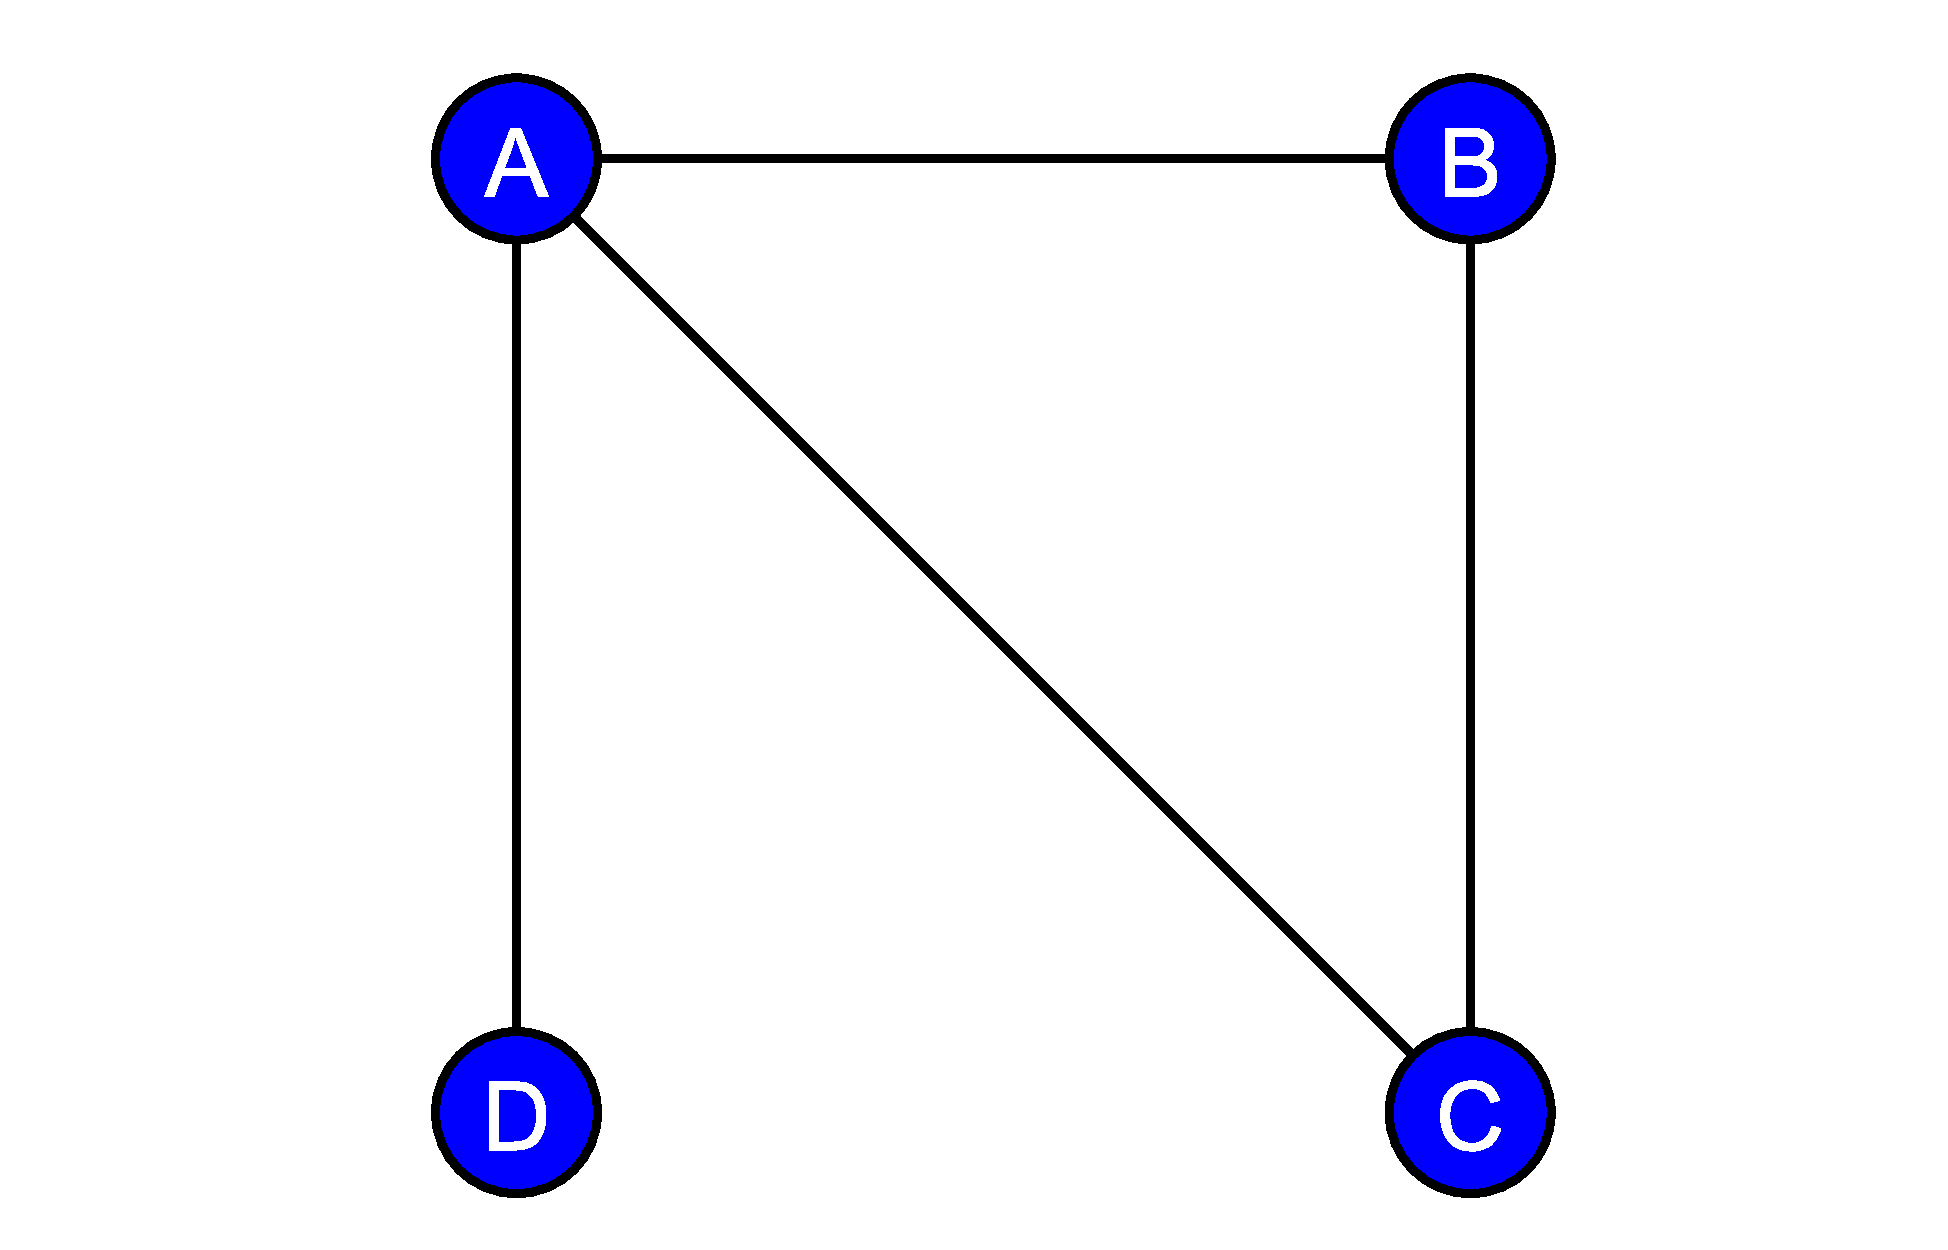
\includegraphics[width=60mm, keepaspectratio]{figures/clustering.pdf}
	\caption{An example graph for illustrating the calculation of the clustering coefficient metric.}
	\label{fig:clustering}
\end{figure}

\subsubsection{Betweenness Centrality}

The betweenness centrality of an node $n$ is quantified by the number of shortest paths that include $n$ as an intermediate node, divided by the entire number of shortest paths. Consequently, this metric is normalized between 0 and 1.

To demonstrate with an example, assume that we searched the following shortest paths denoted by $P_i$:
\begin{itemize}
	\item $P_1 = (v_1, v_3, v_4, v_6, v_5)$
	\item $P_2 = (v_2, v_3, v_4, v_5)$
	\item $P_3 = (v_4, v_3, v_5)$
\end{itemize}

The entire number of shortest paths is equal to 3, and the intermediate nodes are $v_3$, $v_4$ and $v_6$. The betweenness centrality values of the nodes---denoted by $B_i$---are the following:
\begin{itemize}
	\item $B_3 = 1$, since $v_3$ appears in all three paths.
	\item $B_4 = \frac{2}{3}$ due to $v_4$ appears in two paths---$P_1$ and $P_2$. Note that $v_4$ in $P_3$ is the initial node and not an intermediate node.
	\item $B_6 = \frac{1}{3}$
	\item $B_1 = B_2 = B_5 = 0$, since they do not appear in the paths as intermediate nodes.
\end{itemize}
\subsection{Network Topologies} \label{sec:topologies}

In the following sections, we introduce the graph topologies that are relevant to our work. Besides their generation algorithms, we also emphasize the degree distributions they follow.

\subsubsection{Random Graph}

The main concept of the random graph is to create the connections among nodes independently from each other, meaning that the occurrence of an edge between the nodes is not influenced by the other edges. 

Two well-known algorithms exist to create random graphs. The first is the $G(N, M)$ model of Erdős-Rényi~\cite{erdos_random}, and the second is the $G(N,p)$ model from Gilbert~\cite{gilbert_random}. The former means that precisely $M$ edges exist among $N$ vertices, and the latter implies that---in the generation algorithm---every pair of nodes becomes adjacent with $p$ probability. The degree distribution of random graphs follows a Poisson distribution.

\subsubsection{Small-World Model of Watts-Strogatz}

A graph follows a small-world property if the graph has a high average clustering coefficient and small average length of shortest paths.
%todo citation?

The generation algorithm of the Watts-Strogatz topology addresses the creation of networks with small-world properties. The algorithm is constructed as follows: initially, the algorithm creates a ring of $N$ number of isolated nodes, which is equal to the entire number of nodes in the graph. In the second step, every node becomes adjacent to $K$ number of their neighbors, thus creating a lattice graph~\cite{lattice}. This implies that every node has a degree $K$, therefore, its degree distribution fits to a uniform distribution. Besides the variables $N$ and $K$, another parameter appears in the algorithm, the $p$ probability variable. After creating $N$ nodes and $N \cdot K$ connections, every edge is rewired by $p$ probability and attached to a new, randomly chosen node. Note that the two extremes, $p=0$ and $p=1$ entails we obtain a mapping between a lattice and a random graph. As a result, the degree distribution of the Watts-Strogatz model deviates between uniform and Poisson.

\subsubsection{Scale-Free Model of Barabási and Albert}

The scale-free model of Barabási and Albert addresses the generation of a network that follows a power-law degree distribution and includes a small proportion of nodes that have significantly higher degrees than the average. These types of vertices are often referred as \textit{hubs}.

The generation algorithm creates nodes incrementally and connects them to $m$ disjunct nodes. However, instead of choosing nodes randomly, these new connections per nodes are determined by a \textit{preferential attachment}. When the algorithm creates a new vertex then the probability $p_i$ that this vertex becomes adjacent to an $i$ node is:
\begin{align}
	p_i = \frac{d(i)}{\sum_j d(j)}
\end{align}
where $d(i)$ denotes the degree of the $i$ node, and $j$ symbolizes the other existing nodes. As a conclusion, the probability of a node becomes adjacent to another one depends on the degree of the latter. If a higher degree belongs to a node than the average, the probability also increases that the node obtains more connections.
\subsubsection{Hierarchical Network}

The hierarchical network topology~\cite{hierarchical} is generated by a recursive algorithm illustrated in Figure \ref{fig:hierarchical_generation}. Initially, the $0.$ iteration constructs a $K_5$ complete graph\footnote{The diagonal nodes are also connected to each other}, called \textit{cluster}. In the first iteration, the algorithm creates four replicas of the $K_5$ cluster. In the second step in this iteration, the algorithm connects the peripheral nodes from the replicas to the center node. The generation can be continued recursively, as in every $i.$ run, the result graph of the $i-1$ iteration is cloned and the peripheral nodes---the \textit{deepest} vertices in the replicas---are attached to the center node.\\
Finally, the generated hierarchical graph follows a heavy-tail power-law degree distribution, since the graph includes such nodes that have significantly larger degrees---the center nodes---and the probability that these nodes appear is considerably small.

\begin{figure}[!ht]
	\centering
	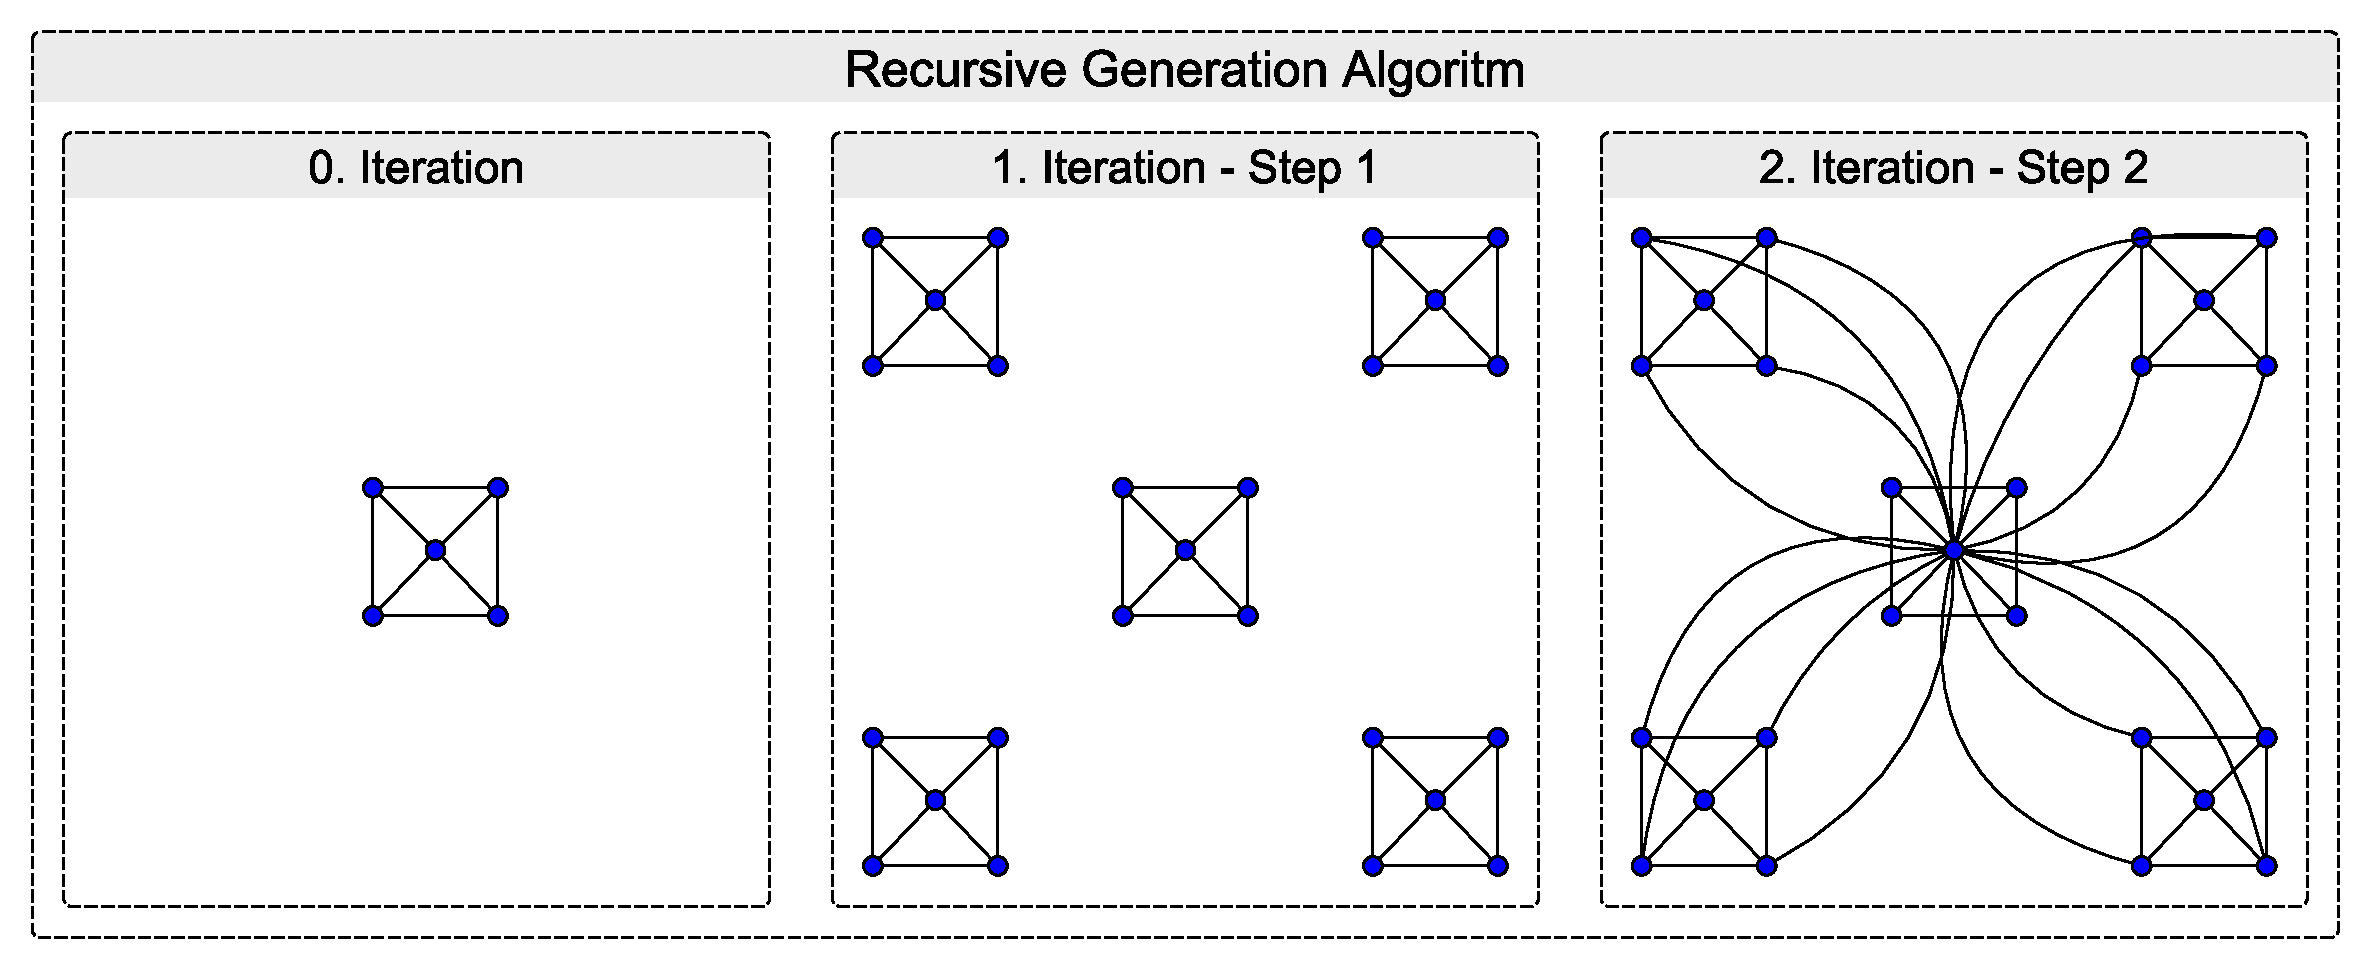
\includegraphics[width=140mm, keepaspectratio]{figures/hierarchical_generation.pdf}
	\caption{The first iteration in the recursive generation algorithm of the hierarchical network.}
	\label{fig:hierarchical_generation}
\end{figure}

	\chapter{Related Work}


\section{Benchmarks of NoSQL Databases}

A wealth of literature is available related to the performance comparison of different NoSQL databases over RDF data. Instead of introducing a part of these papers, we focus on the foundations of the measurements, the benchmark frameworks. In the following, each section represents a benchmark particularly connecting to RDF data models. Finally, Section \ref{sec:benchmark_conclusions} compares the frameworks, and by drawing conclusions based on the benchmarks, it also contains the main concepts on which we will rely in our search.

\subsection{Yahoo!~Cloud Serving Benchmark}

The \textit{Yahoo!~Cloud Serving Benchmark} was elaborated in order to compare performance of the new generation
of cloud data serving systems~\cite{ycsb}. The framework proposes different workloads by assigning
different distributions to them that determine the operation to perform --- get or put --- and the record from the data model to be read or written. In other words, the particular distributions specify the exact numbers of read or update queries in a workload, and also affect the choosing of records on which the workload operates. In order to demonstrate, Figure 1 %todo insert pic from 5
represents the available distributions and number of choices per records.

\subsection{Berlin SPARQL Benchmark}

The Berlin SPARQL Benchmark (from now on BSBM) is settled in an e-commerce use case in which a set of products
is offered by different vendors and consumers have posted reviews about these products on various review sites~\cite{berlin}. Taken scalability into consideration, BSBM proposes an arbitrary increased model size. Similarly to YCSB, BSBM concentrates on read and update operations as well, as it defines three different use cases and a suite of benchmark queries in each of them~\cite{berlin_specification}. The queries were elaborated to simulate realistic, real-life workloads.

In contrast to YCSM, BSBM defines particular performance metrics that relate mainly to the query execution times from different perspectives. For example, the most important metrics are the following:
\begin{itemize}
	\item{Queries per Second}: It equals to the number of queries that executed properly by the system within a second.
	\item{Query Mixes per Hour}: Denotes the number of \textit{mixed} queries with different parameters that evaluated within an hour.
	\item{Overall Runtime}: The overall time that a certain amount of query mixes required.
\end{itemize}


\subsection{DBpedia SPARQL Benchmark}
DBpedia SPARQL Benchmark proposes datasets in various sizes derived from the DBpedia~\cite{dbpedia_data} knowledge base, and perform measurements on real queries that were issued against existing RDF data~\cite{dbpedia}. Similarly to BSBM, DBpedia also defines metrics to provide a more precise performance analysis. These are the same as in the case of BSBM: \textit{Query Mixes per Hour}, and \textit{Queries per Second}. Furthermore, DBpedia investigates the characterization of the models as well and calculates the average in- and outdegree, the number of nodes and distinct IRIs, however, it uses these measurements to judge and maintain the generated model to be similar to the original data set. As a consequence, DBpedia does not explore model and performance correlations neither.

\subsection{SP$^2$Bench}
The SPARQL Performance Benchmark (SP$^2$Bench) is designed to test the most common SPARQL constructs,
operator constellations, and a broad range of RDF data access patterns~\cite{sp2bench}. Instead of defining a sequence of use case motivated queries, the framework proposes various queries that cover specific RDF data management approaches.

SP$^2$Bench is based on the \textit{Digital Bibliography and Library Project} (commonly known as \textit{dblp}) which provides an open bibliographic information on major computer science publications~\cite{dblp}. The benchmark queries are not explicitly evaluated over the \textit{dblp} dataset, since SP$^2$Bench uses arbitrarily large, artificially generated models for the measurements, however, these models are constructed to follow real-life characteristics that were found in the original \textit{dblp} dataset, such as a power-law distribution.

Similarly to BSBM, SP$^2$Bench also measures additional performance related metrics besides execution time, such as disk storage cost, memory consumption, data loading time, success rates, and every one them captures different aspects of evaluations.


\subsection{Train Benchmark Framework}

\begin{figure}[!ht]
	\centering
	\includegraphics[width=150mm, keepaspectratio]{figures/functionality.pdf}
	\caption{An overview of Train Benchmark.}
	\label{fig:functionality}
\end{figure}

Short overview: well-formedness constraints + model validations, transformations.\\
Extended scope: RDF, EMF, SQL, Graphml.
Domain disadvantages. Emphasize this as common problems.

What is not mentioned: workflow, components, tools, detailed generator


The original domain of the Train Benchmark framework (introduced in \ref{section:metamodel} is not applicable for our goals to analyze graph queries, and study model - performance relationships. The main problems connecting to the domain are summarized in the following list:
\begin{enumerate}
	\item The original domain is not related to a real-life model, which leads to the fact that the cardinalities of the elements and their relationships do not follow a real model's characteristic, therefore, the measurement results of different tools cannot be claimed to be representative in a real-life use case. \label{item:railway_problem1}
	\item Besides the origin of the domain, the second problem is that the artificially generated models do not cover a well-known topology or degree distribution that can be observed in actual networks. \label{item:railway_problem2}
	\item Finally, the generated models of Train Benchmark are not capable of attaching arbitrary connections between the elements. \label{item:railway_problem3}
\end{enumerate}

Obviously, problem \ref{item:railway_problem2} is relevant to the generator component's insufficiency, since a representative distribution can be achieved independently on the domain, however, in order to generate arbitrary distributions, it is essential to guarantee a solution for problem \ref{item:railway_problem3}.

Problem \ref{item:railway_problem3} requires some explanation. In order to construct graphs with different degree distributions, it is an essential expectation of the domain to contain self-references, thus indicating that any of the vertices can be adjacent. In addition, the presence of a self-reference should be also interpretable conceptually in the domain. 

Considering the original domain, the type \textsf{Segment} represents the majority of the elements, however---without breaking the original meaning of the domain---we cannot make connection between any of the segments.


To summarize, a new domain is necessary that is related to a real-life model, and also suited to use for generating different distributions.


\subsection{Conclusions} \label{sec:benchmark_conclusions}

One common attribute of the previously introduced benchmark frameworks is that they lack precise analysis of searching connection between model characteristic and evaluation performance. In these frameworks, it is not supported to assess a tool's performance on different topologies, still using the same domain. Generally, the frameworks propose the generation of variously large models, thus investigating scalability, however, they do not focus on modifying the internal structures of the models, and generate different topologies, even in the same size.

%todo more? metrics? prob dist? use case?

	\chapter{Overview of the Approach}

\section{Main Concepts}

Our main goal is to provide a benchmark framework for analyzing model and performance relationships in an arbitrary workload, and characterizing  the performance quantitatively with model related metrics.

Our concept includes the following systems illustrated in Figure \ref{fig:frameworks}. We rely on two existing frameworks in our work, the Train Benchmark and the MONDO-SAM framework, and we elaborate \framework, the \textit{MONDO-Metrics-Based Analysis of Performance} framework.
%todo mondom sam cite
\begin{figure}[!ht]
	\centering
	\includegraphics[width=130mm, keepaspectratio]{figures/frameworks.pdf}
	\caption{An overview of the frameworks in our approach.}
	\label{fig:frameworks}
\end{figure}

\paragraph{MONDO-SAM}
The MONDO-SAM framework was created under the project MONDO~\cite{mondo} with the motivation to provide a common benchmark framework in Model Driven Engineering (MDE) for benchmark developers. MONDO-SAM can be considered as an abstract layer that proposes an evaluation engine to execute arbitrary workflows independently on the current workload. MONDO-SAM also guarantees the serialization and data visualization of the benchmark results.

\paragraph{Train Benchmark}
The Train Benchmark framework is based on the evaluation engine provided by MONDO-SAM, and it proposes a benchmark for measuring model validations and transformations, introduced in Section \ref{sec:train}.

\paragraph{\framework}
As Figure \ref{fig:frameworks} depicts, our new framework---\framework---also relies on the evaluation engine located in MONDO-SAM, furthermore, it uses a part of the components in Train Benchmark that are adequate for our purpose as well.


The fundamental goal of \framework~is to find model metrics that are suited to characterize the performance of query evaluations with respect to an arbitrary query and tool. By generating artificial graphs with various characteristics and obtain a fluctuation in their descriptive metrics, we are able to show a quantitative relationship between model metrics and performance.
%todo picture

Figure 222 illustrates the main concept of our work. The \framework~framework generates different graph topologies which show significant deviations in metrics. These topologies are the following:
\begin{itemize}
	\item Random graph
	\item Small-world model of Watts-Strogatz
	\item Scale-free Network of Barabási-Albert
	\item Hierarchical Network
\end{itemize}
After calculating the descriptive metrics belonging to the models, the benchmark framework evaluates the queries on each model in the particular databases and assess the evaluation times. It analyzes the results and creates regression models to explore the relationships between the variables.

\subsection{Use Cases}

\framework~proposes a benchmark to explore that a particular tool is how sensitive to the underlying graph topology and the variation of metrics. This knowledge can be utilized among tool developers, since a significant alteration between the graphs implies a comprehensive

main approach with figure
mondo-sam: benchmark engine, execution of phases, publishing, reporting framework
mondo-mbpal: domain independent framework for performance analysis based on metrics: model metrics, model generation different characteristics, topologies, regression analysis
trainbenchmark: use come components
British railway domain


the difficulty of using existing real-life domains. cannot illustrate scalability or particular distribution between metrics -> must generate artificial models like anybody else does.

British model characteristics generator: dbpedia, sp2bench
from the model based and make deviations in generated models
different topologies, investigate the metrics impact to the performance, concentrate on this




The main idea of our work and its possible utilization is depicted in Figure 1121212. %todo create overview optimization figure
In the first step, the framework analyzes the graph-based models and explores their characteristics, secondly, it evaluates the queries on the models and measures the performance---so the evaluation time. In the next step, the evaluation times and the corresponding model characteristics are analyzed together, as the framework searches relationships between them. The goal is to find that how the characteristics of the models impact the performance of the queries.

As Figure 11212 %todo reference
illustrates as well, a possible utilization of our approach is the field of query optimization. Based on the analysis results from the framework, it becomes feasible to choose an appropriate optimization technique for a particular tool in the light of the model and performance relationship.

Three challenges can be found in our research. At first, we have to provide a solution for our framework to generate models with different characteristics that impact the performance of a certain query and thus cause a deviation in evaluation time. Secondly, we have to find model attributes that are able to characterize the models individually. Furthermore, these attributes must be suitable to create quantitative relationships among them and the evaluation times.


link this and the following sections
find individual attributes of models that can cause performance fluctuation, what is main indicator that distinguishes the graphs?

\section{Models and Metrics}
\subsection{Real-Life Networks}

%todo copy heavy tail to background
In the discipline of graph theory, the internal structures of real-life networks are comprehensively investigated. The main approach in the analysis of these networks is to explore the degree distributions and study the specific metrics---typically the clustering coefficients, average degrees, average shortest paths---that are suited to characterize the graphs appropriately. Based on the degree distributions and metrics, one can draw conclusion how a particular real-life network shows a similar characteristic to the well-known topologies such as the random graph, scale-free model, small-world model of Watts-Strogatz, or hierarchical network.\\
For example, the network of world-wide-web is studied in~\cite{www1} and~\cite{www2} as well, and the authors observe that the degree distribution of the \textit{www} follows a power-law distribution with a heavy tail\footnote{The concept of heavy tail means that there is a larger probability of receiving significantly higher values, than it is normally expected~\cite{heavy_tail}.}, which indicates the presence of web pages with significantly higher degrees than the average degree. Since the probability of occurrences of these web pages is considerably low, the connectivity of the world-wide-web can be represented by the scale-free model of Barabási and Albert.

%todo insert table from StatisticalMechanics_Rev of Modern Physics 74, 47 (2002)

More examples can be found in the study of Barabási and Albert~\cite{statistical_mechanics}, as they review the advances of different publications and investigate the characteristics of different real-life networks (Table). Empirical results prove that the \textit{movie actor collaboration network}, \textit{cellular networks}, \textit{phone call} and \textit{citation} networks also follow power-law distributions. Many of the studied networks can be considered as scale-free models, however, a part of these graphs---for example the network of movie actors---also show small-world properties and high clustering coefficient in their connectivity similarly to the Watts-Strogatz or hierarchical topology.

As far as the Watts-Strogatz model---and the random graph\footnote{The topology of Watts-Strogatz is actually considered as a bridge between a lattice and a random graph based to its $p$ probability value. Thus, according to $p$, the WS model shows uniform or Poisson distribution.}---are concerned, their specific degree distribution---Poisson---rarely appears in the real-life networks, as it is emphasized in~\cite{random_study}. Actually, none of the artificial topologies can be identified perfectly to real-life models, however, the ensemble of the specific attributes of these well-known topologies are frequently appear in them. As a conclusion, we conjecture that the characteristics belonging to the well-known topologies are the foundations of our solution, namely, finding those representative metrics of graphs that are suited to characterize not only the model appropriately, but the relationship between model and performance as well.

\subsection{Network Topologies and Representative Metrics}

Barabási and Albert inspect the natures of the well-known graph topologies in~\cite{statistical_mechanics}, such as the random graph, scale-free and the Watts-Strogatz model. As a main result, they observe that there are significant differences among the topologies regarding specific graph metrics. Based on their study and the research of hierarchical graphs~\cite{hierarchical}, the following metric deviations are assumed	between the four topologies, illustrated in Table \ref{tab:topology_metrics}. The random graph is considered as a reference point, and every value is compared to its metrics by assuming that the networks are in the same size.
\begin{table}[ht]
	\footnotesize
	\centering
	\begin{tabular}{ l c c c c}
		\toprule
		Metric & Random & Hierarchical & Scale-free & Watts-Strogatz \\ 
		\midrule 
		\textbf{Max Degree} & $\bullet$ & $\bullet$$\bullet$$\bullet$ & $\bullet$$\bullet$$\bullet$ & $\bullet$ \\ \hline
		\textbf{Clustering Coefficient} & $\bullet$ & $\bullet$$\bullet$$\bullet$ & $\bullet$ & $\bullet$$\bullet $\\ \hline
		\textbf{Avg Shortest Path Length} & $\bullet$ & $\bullet$$\bullet$ & $\bullet$ & $\bullet$$\bullet$ \\ \hline
		\bottomrule
	\end{tabular}
	\caption{Graph topologies and their descriptive metrics}
	\label{tab:topology_metrics}
\end{table}
%todo describe bullets in detail
As Table \ref{tab:topology_metrics} demonstrates, each topology can be characterized by different metric values, which leads to the assumption that if the diversity between the topologies may cause fluctuations in the performance of a particular query evaluation, then these metrics are adequate to characterize the model and performance relationships quantitatively.

%todo use lattice ref in background
%todo emphasize lattice, random and p value in background, maybe add a picture as well

However, the values of metrics in Table \ref{tab:topology_metrics} are misleading due to the reason that the metrics of the Watt-Strogatz model highly depend on the initialization of the network, namely, the value of $p$ probability that is used in the generation.

\begin{figure}[!ht]
	\centering
	\includegraphics[width=100mm, keepaspectratio]{figures/ws_metrics.png}
	\caption{Characteristic path length $L(p)$ and clustering coefficient $C(p)$ of Watts-Strogatz model}
	\label{fig:ws}
\end{figure}

By modifying $p$, the Watts-Strogatz model represents a bridge between a lattice and a random graph. As Figure \ref{fig:ws} illustrates\footnote{The original figure can be found in~\cite{ws_metrics}.}, the clustering coefficient ($C(p)$) and average shortest path ($L(p)$) metrics are changed with respect to $p$ scaling. The values are normalized by $L(0)$ and $C(0)$ that represent the clustering coefficient and average shortest path metrics for a lattice graph. As a conclusion, the Watts-Strogatz model shows significant deviations in these two metrics in the light of the $p$ probability value. 

%todo add betweenness reference to background
Besides the models in Table \ref{tab:topology_metrics}, the metrics also require modifications. The problem is that the maximum degree metric alone does not include a comprehensive information about the internal structure of the network, since it does not emphasize the role of a node with maximum degree in the connectivity of the graph. Hence, we introduce another metric---the \textit{betweenness centrality}---which characterizes adequately the importance of a higher degree, since the higher value of betweenness centrality belongs to a vertex, the more shortest paths include that node, symbolizing that node represents the center in the graph.

After these minor modifications, the topologies and the related metrics are showed in the extended Table \ref{tab:topology_metrics2}. The \textsf{WS-x} abbreviations symbolize the Watts-Strogatz models indicating that the $p$ value is equal to $x$. The values of the betweenness centrality are determined by our initial conjecture considering that the center node in a hierarchical network and the \textit{hubs} in a scale-free model may occur more times in the shortest paths due to the fact that they have higher degrees. The main conclusion is that we can achieve a higher deviation among the metric values by using these topologies, and thus, in the following we concentrate on these networks.
\begin{table}[ht]
	\footnotesize
	\centering
	
	\begin{tabular}{ l c c c c c c}
		\toprule
		Metric & Random & Hierarchical & Scale-free & WS-0.1 & WS-0.01 & WS-0.001 \\ 
		\midrule 
		\textbf{Max Degree} & $\bullet$ & $\bullet$$\bullet$$\bullet$ & $\bullet$$\bullet$$\bullet$ & $\bullet$ & $\bullet$ & $\bullet$ \\ \hline
		\textbf{Clustering Coefficient} & $\bullet$ & $\bullet$$\bullet$$\bullet$ & $\bullet$ & $\bullet$$\bullet$ & $\bullet$$\bullet \bullet$ & $\bullet$$\bullet$$\bullet$\\ \hline
		\textbf{Avg Shortest Path Length} & $\bullet$ & $\bullet$$\bullet$ & $\bullet$ & $\bullet $ & $\bullet \bullet$ & $\bullet$$\bullet$$\bullet$\\ \hline
		\textbf{Betweenness Centrality} & $\bullet$ & $\bullet$$\bullet$$\bullet$ & $\bullet$$\bullet$ & $\bullet$ & $\bullet$ & $\bullet$\\ \hline
		\bottomrule
	\end{tabular}
	\caption{Graph topologies and their descriptive metrics with extensions}
	\label{tab:topology_metrics2}
\end{table}

\section{Metric and Performance Comparison}

Showing an appropriate performance and metric relationship is an essential part of our approach. The first notion is the search of correlations between the metrics and performance.

A similar problem is studied in~\cite{algebraic1} and~\cite{algebraic2}, where the authors generate well-known topologies and inspect the connectivity and robustness of the networks. In their case, a network is said to be robust if its performance is not sensitive to the changes in topology. In~\cite{algebraic1}, the algebraic connectivity metric is studied to search robustness and metric relationships, however, they show that the algebraic connectivity is not trivially correlated to the robustness of the network.\\
The authors in~\cite{algebraic2} investigate the impact of betweenness centrality, algebraic connectivity and average degree to robustness, and they also draw the conclusion that there is no unique graph metric to satisfy both connectivity and robustness objectives while keeping a reasonable complexity, since each metric captures some attributes of the graph.

Partly based on the advances of these two publications and our initial assumption of the topologies and their metrics (Table \ref{tab:topology_metrics2}), we expect that we cannot find a correlation between one metric and the performance, hence, we conjecture that only the ensemble of more metrics is suited to find relationship.

In order to find quantitative connections, we use regression analysis to show how the various metrics impact the performance. 

\subsection{Sample Choosing}

By using regression analysis on a sample, it is inevitable to regard the sample to be unbiased. In our case, a bias in a sample of graph topologies means a fluctuation in the size of the models. Obviously, one topology in the sample with larger amount of nodes can bias the connection between the models and the performance, therefore, our framework must support the generation of \textit{uniform} models with respect to the amount of nodes and edges, even in the case of different topologies as well.\footnote{From now on, under the concept of uniform models we mean models with approximately equal number of nodes and edges, despite the diversity of their internal structures.}

The number of nodes in a graph is the most dominant factor to the performance

\section{Usage of the Train Benchmark Framework}
%todo rewrite
For our approach, we use the Train Benchmark framework to generate different topologies, evaluate queries on the models, and finally, analyze the results by creating regression models to show how the model metrics characterize the performance.

Since our research partly deviates from the field that the Train Benchmark investigates, it is necessary to extend the framework for our purpose. To eliminate the limitations of the framework (described in Section \ref{sec:railway}), we elaborate a new generation component based on a real-life model and enhance the framework with model and performance analysis.

	\chapter{Contributions}

In the following sections, we present the main contributions related to the \framework~framework and the Homogeneous Graphs Benchmark.

\section{Overall Architecture}

Figure \ref{fig:architecture} depicts the frameworks and the main components belonging to them, additionally, it also denotes which components are reused from Train Benchmark. All of the frameworks and their components were elaborated in Java programming language.

\begin{figure}[!ht]
	\centering
	\includegraphics[width=150mm, keepaspectratio]{figures/architecture.pdf}
	\caption{The architecture of our approach.}
	\label{fig:architecture}
\end{figure}

In the following, we introduce the components.

\paragraph{Benchmark Engine}
The \textsf{Benchmark Engine} in MONDO-SAM is responsible for evaluating an arbitrary sequence of phases consecutively. A phase is considered as the atomic execution unit in a benchmark. The engine also measures the evaluation times of phases, hence, it is the component that measures the performance of query evaluations in our work.

\paragraph{Analyzer Components}

The \textsf{Model} and \textsf{Query Analyzer} units belong to the \framework~framework and define an interface for the metrics calculation. The \textsf{Model Analyzer} investigates the model related metrics, and the \textsf{Query Analyzer} relates to the query definitions. As it can be observed, the concrete metric calculations---\textsf{RDF Model Analyzer} and \textsf{RDF Query Analyzer}---appear in the HG Benchmark.

\paragraph{Metrics}

The definitions of \textsf{Model Metrics} can be found in \framework. The model metrics symbolize graph metrics with applying the commonly used naming conventions from graph theory. Note that the HG Benchmark does not contain further RDF-based metrics implying that we use the graph-based naming conventions in our work.

\paragraph{Generators}

The generator components belong to the HG Benchmark. The abstract \textsf{Generator} unit is utilized from Train Benchmark. The \textsf{Stations Generator} component is responsible for transforming the real-life British Railway Stations model to RDF. Last, the \textsf{Topology Generators} construct different homogeneous graphs fitting to well-known topologies and transform them to RDF format.

\paragraph{RDF Driver}
The \textsf{RDF Driver} manages the connections between the measured RDF databases and the benchmark framework, furthermore, it also accomplishes the loading of the models. 

\paragraph{Query Executor and Query Builder}

The query evaluations are initiated by the \textsf{Query Executor} component. The \textsf{Query Builder} is responsible for creating and altering the query definitions in runtime.

\section{British Railway Stations}

In order to test our regression models on an entirely different graph, we introduce a real-life model to our work. We use a model of train stations provided by the \textit{Network Rail} company that runs, maintains, and develops Britain's rail tracks~\cite{network_rail}. Network Rail publishes a number of different data available to developers, one of them is a \textit{daily extracts and updates of train schedules}~\cite{schedules_data} that which formed the basis of our data set.

The data contains approximately 10~000 British stations that belong to train schedules as destinations. We concentrate on the network of stations, and map it to a graph where every vertex symbolizes a station. An edge is drawn between two nodes---\ie two stations---if these stations appear consecutively in a destinations path belonging to a schedule.

\section{Uniform Model Generation}\label{sec:uniform_generation}

It is an essential requirement of the HG Benchmark to guarantee uniform model generation among the topologies indicating the same size of the generated models. We propose a model generation technique to generate topologies with the same amount of nodes and edges.

\subsection{Number of Nodes}

The random graph and the Watts-Strogatz model are constructed by initializing $|V| = N$ number of vertices, and then the algorithms determine which one of them become adjacent. In the scale-free model generator, the nodes are created incrementally until $|V| = N$, and a precise number of nodes can be obtained regarding these topologies.

The only problem about generating topologies with a certain number of nodes is the recursive algorithm of the hierarchical graph, which algorithm has to be terminated.

\subsubsection{Termination of the Hierarchical Network Generation Algorithm}\label{sec:hierarcical_contribution}

Since the generation of hierarchical network is recursive instead of being incremental---as in the case of the three other topologies---it is necessary to determine a termination from the recursive algorithm. The termination point is evident, as soon as the number of created nodes reaches the limit, the algorithm has to be stopped. However, it cannot be predicted in which phase the algorithm stops exactly. As a consequence, the possible problems have to be managed.

\begin{figure}[!ht]
	\centering
	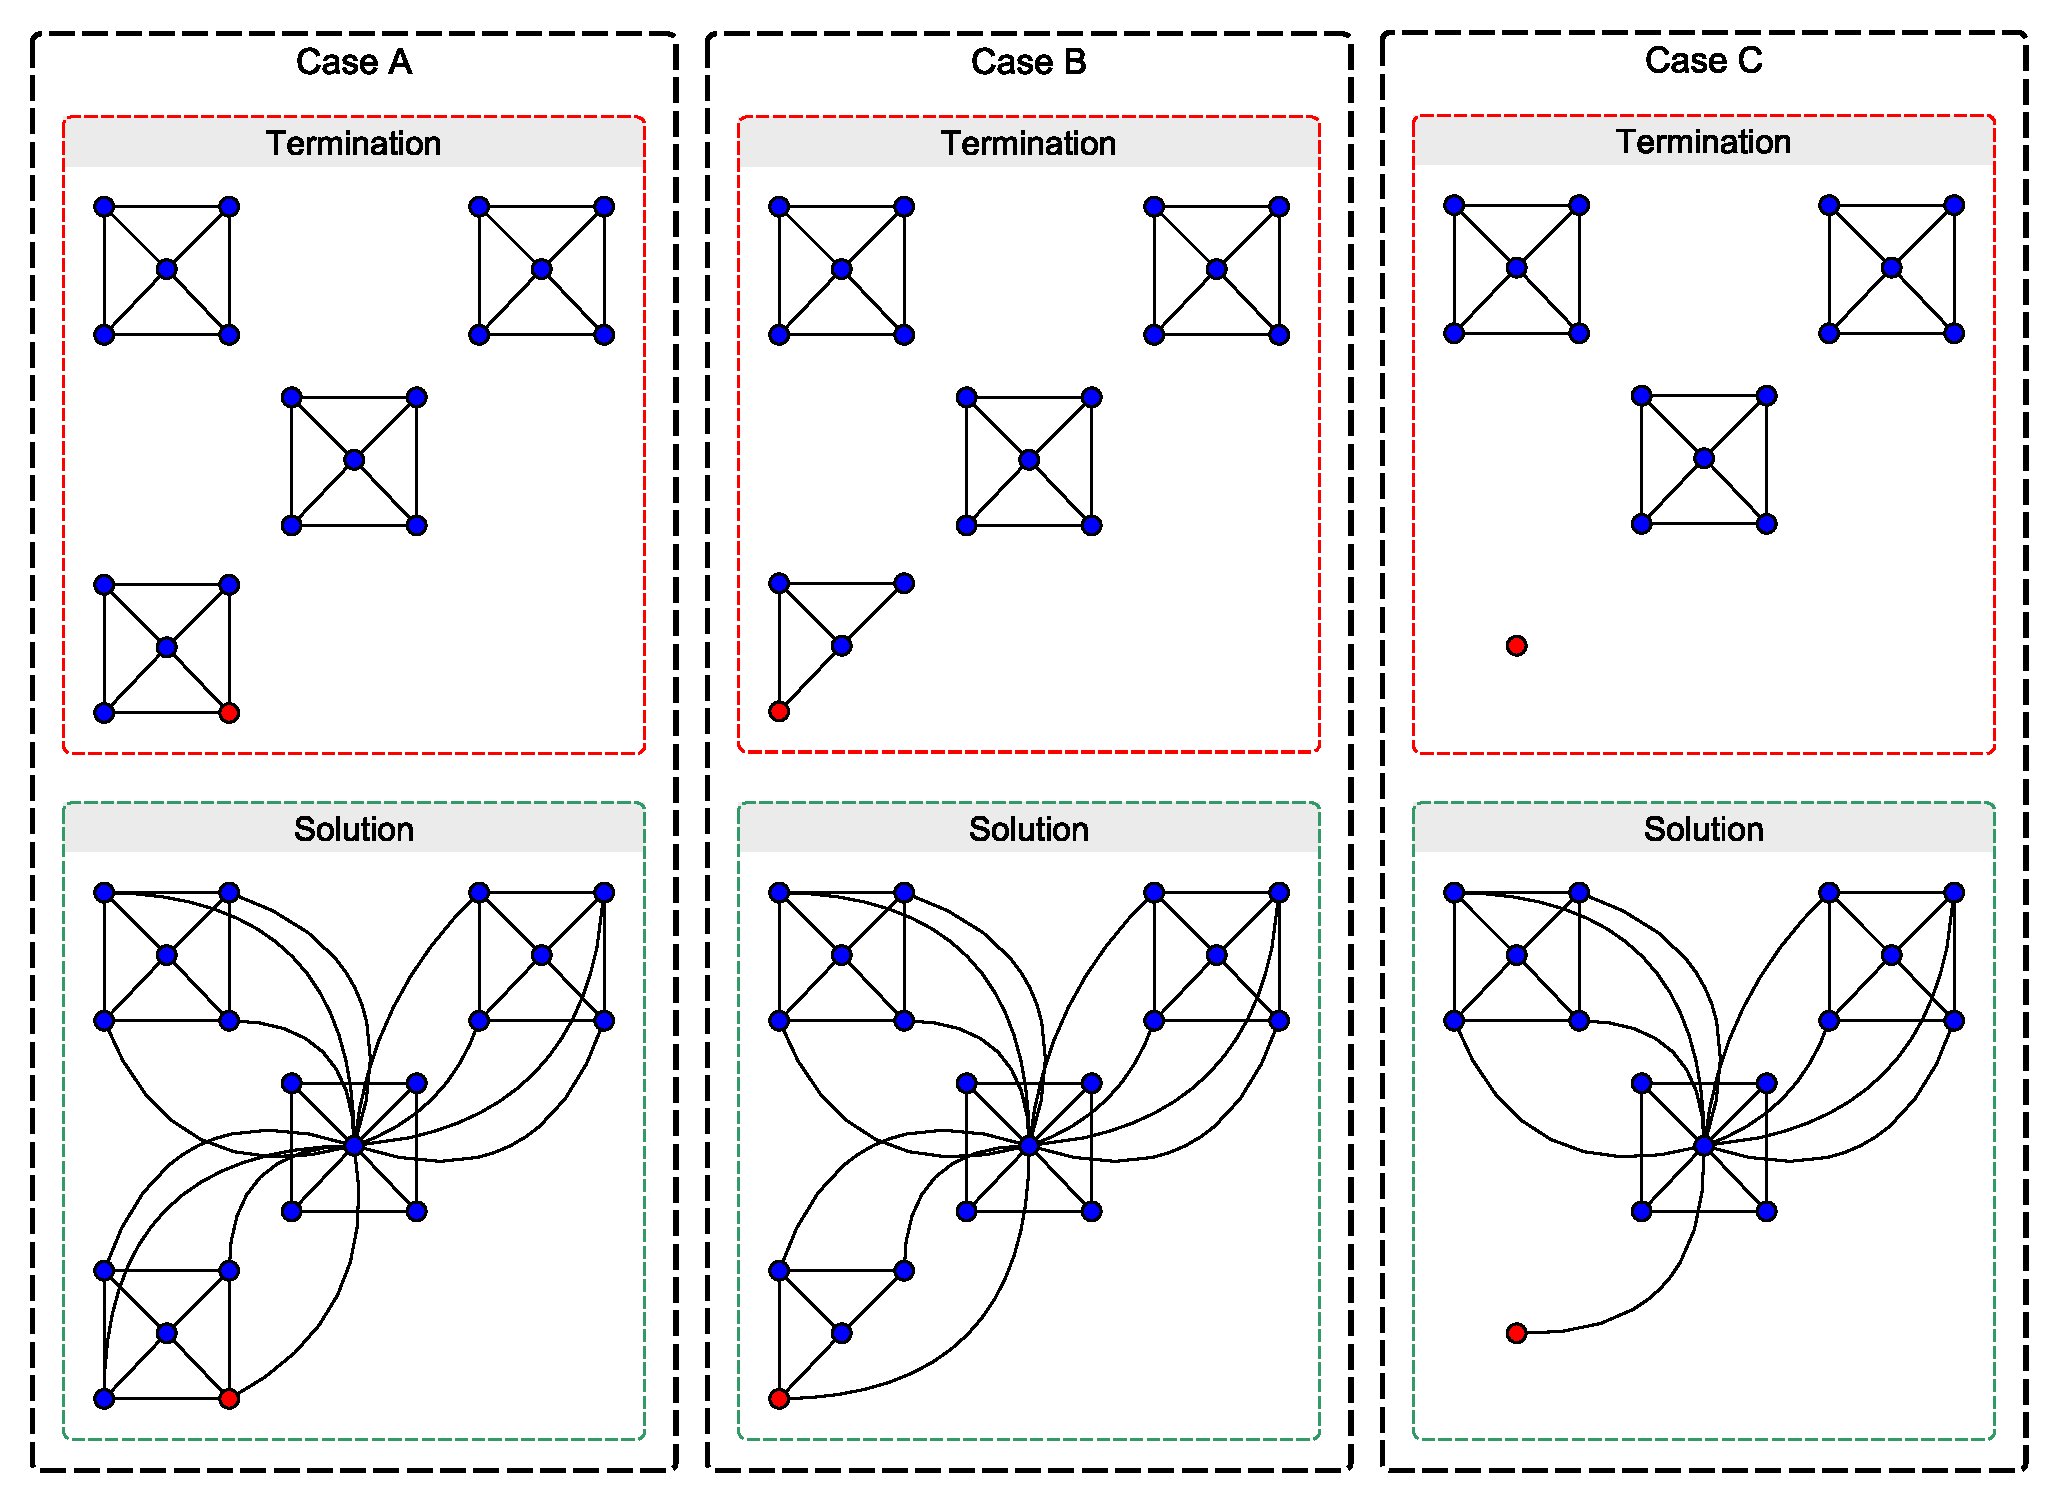
\includegraphics[width=150mm, keepaspectratio]{figures/hierarchical.pdf}
	\caption{Possible termination problems in the hierarchical graph generation.}
	\label{fig:hierarchical_problems}
\end{figure}

The possible problematic cases are demonstrated in Figure \ref{fig:hierarchical_problems}. In \textsf{Case A}, \textsf{B}, and \textsf{C}, the expected numbers of nodes are 20, 19, and 16, respectively. As it can be observed in these cases, this limit is always reached before the fourth cloning occurs, since 5 clusters should be created with 25 vertices at the end of this step in the recursion.

In the solution in \textsf{Case A}, the generator stops the cloning procedure and connects the diagonals to the center. Regarding \textsf{B}, the termination happens during the generation of a cluster. As a solution, the last cluster becomes partial, and similarly, every diagonal is attached to the center. \textsf{Case C} represents that scenario when the last cluster only consists of one node. To prevent isolation, the last vertex is considered as a diagonal, and be connected to the center.

\subsection{Number of Edges}

%todo note that the diagonal nodes are also connected — links not visible on hierarchical graph
In terms of the random graph, scale-free, and WS model, their generation algorithms can be adjusted arbitrarily, meaning that an optional number of nodes or edges can be achieved. As a matter of fact, reaching a certain amount of nodes or edges in these networks are handled separately.

Unfortunately, the creation of nodes and edges in the hierarchical graph occur together. Since the amount of edges depends on the number of nodes and iterations in the recursive algorithm, it cannot be configured arbitrarily. A solution is that we adjust the other topologies to have the same number of edges as the hierarchical model. This solution requires to calculate the exact number of edges in a hierarchical network with respect to the iteration.

\subsubsection{Estimating the Number of Edges in Hierarchical Graphs}

The literature relating to hierarchical graphs does not mention the exact number of edges or its correlation to the amount of nodes, hence, we propose a solution to estimate $|E|$ in the recursive algorithm for every iteration.

At first, let us define the necessary variables hereunder:
\begin{itemize}
	\item{$i$}: represents the current iteration in the original hierarchical algorithm.
	\item{$c$}: indicates the number of clones in every iteration.
	\item{$n$}: the cluster size is denoted by $n$, which is a $K_n$ complete graph.
	\item{$F_i$}: indicates the constructed graph after the $i.$ iteration. %todo why F? maybe change it to H later
	\item{$|E_{F_i}|$}: the number of edges of $F_i$.
\end{itemize}

The algorithm works as follows. In the 0.~iteration, the hierarchical graph consists of one $K_n$ cluster. Formally, $F_0 = K_n$, and $|E_{F_0}| = |E_{K_n}| = \frac{n \cdot (n-1)}{2}$. In the 1. iteration, the algorithm clones $F_0$ $c$ times, and connects the peripheral nodes from each $F_0$ to the center node. It entails that 
\begin{align}\label{eq:f1_version1}
	|E_{F_1}| = (c+1) \cdot |E_{K_n}| + c \cdot (n - 1)	
\end{align}
since $c+1$ number of $K_n$ can be found in $F_1$, and $c \cdot (n - 1)$ edges can be drawn from the $c$ number of replicas to the center.

Note that in the first iteration $K_n$ can be substituted with $F_0$, and the algorithm in the first part of the $i.$ iteration creates $c$ replicas of the result of the $i-1.$ iteration, namely, $F_{i-1}$. In the second part of the $i$ iteration, the algorithm connects the clusters from the cloned replicas to the center node. These connections are made between the peripheral nodes in each replica and the center, which indicates that in the $i.$ iteration the algorithm connects $n-1$ peripheral nodes from $c$ number of replicas of $F_{i-1}$. Due to $F_{i-1}$ includes $c^{i-1}$ number of clusters, we obtain

\begin{align}\label{eq:fi_formula}
	|E_{F_i}| = (c+1) \cdot |E_{F_{i-1}}| + c \cdot c^{i-1} \cdot (n - 1)	= (c+1) \cdot |E_{F_{i-1}}| + c^i \cdot (n - 1)
\end{align}

Equation \ref{eq:fi_formula} is equal to the number of edges of a completely finished hierarchical network, however, the generation algorithm in the HG Benchmark is possibly terminated to reach a certain number of nodes which leads to the fact that $|E_{F_i}|$ must be scaled down by the proportion of the maximum ($|V_{F_i}|$) and the required number ($|V_H|$) of vertices. If the hierarchical graph we intend to generate is denoted by $H$, then
\begin{align}\label{eq:h_formula}
	|E_H| = |E_{F_i}| \cdot \frac{|V_H|}{|V_{F_i}|}
\end{align}
where $\frac{|V_H|}{|V_{F_i}|} \leq 1$.

By using Equation \ref{eq:h_formula}, we can calculate the number of edges of a hierarchical graph and configure the other topologies to reach the same quantity.

\subsubsection{Configuring the Random Graph Model}
From the two most well-known algorithms, Gilbert's $G(n,p)$ model is adapted to the framework, which implies that the exact value of $p$ has to be determined from the number of edges in the hierarchical graph, $|E_H|$. Based on~\cite{random_p}, the $p$ probability can be calculated from the number of nodes and edges as follows:
\begin{align}
	p = \frac{|E_H|}{\binom{|V|}{2}}
\end{align}
where $|V|$ denotes the number of nodes.

\subsubsection{Configuring the Watts-Strogatz Model}\label{sec:watts_generation}

Regarding the Watts-Strogatz model, in the beginning of the generation algorithm, $K$ number of consecutive nodes are connected to each other. During the algorithm, by rewiring the edges the amount of $|E|$ is not changed. As a conclusion, in order to achieve a uniform size similarly to the hierarchical graph, $K$ has to be adjusted as $K = \frac{|E_H|}{|V|}$.

Generally, the $K$ value in the algorithm is a constant integer. In order to configure the WS model properly, we extend the algorithm by defining an inclusive lower bound ($K_1$) and upper bound ($K_2$) for $K$, as $K\in[K_1, K_2]$. We also assign a $p$ probability to $K$ that determines the likelihood that $K$ is equal to $K_2$ and $1-p$ to $K_1$. Derived from the equation $K = \frac{|E_H|}{|V|}$, it results in $K_1 = \Big\lfloor\frac{|E_H|}{|V|}\Big\rfloor$ and $K_2 = \Big\lceil\frac{|E_H|}{|V|}\Big\rceil$, additionally, the $p$ probability equals to the fractional part, as $p = \Big\{\frac{|E_H|}{|V|}\Big\}$. Hence, by turning $K$ to a random variable, we can generate WS models with the same number of edges as $|E_H|$.

\subsubsection{Configuring the Scale-Free Model}

The scale-free topology is generated incrementally, since every step a new node is inserted to the graph with $m$ new connections. To obtain $|E_H|$ edges, the $m$ variable has to be configured. This leads to $m = \frac{|E_H|}{|V|}$.

In the original generation algorithm, every new vertex connects to a constant number of disjunct nodes, which indicates that $m$ is a constant integer. Similarly to the notion in the Watts-Strogatz model generation (\ref{sec:watts_generation}), this constant value is converted to a random variable based on a particular probability, derived from $|E_H|$.

\subsection{Possible Model Configuration}

In the artificially generated models the size, topology and density is optionally configurable. 

The size of the model---the number of nodes---is calculated by a formula as $|V| = s \cdot 2^i$, where $s$ is the step size constant and $i$ is a positive integer. It implies that an arbitrary model size can be obtained among the topologies.

Besides the size, the density of the graphs is also configurable, so the number of edges in the topologies. Since the hierarchical network is considered as the reference model due to the uniform model generation, the density parameter calibrates the generation algorithm of the hierarchical graph, namely, the size of the $K_n$ clusters with altering $n$. 

\section{Performance Analysis}

\subsection{Workflow}

A workflow in the HG Benchmark is divided into phases that are considered as the atomic execution units. An arbitrary sequence can be created among the phases, which---during the benchmark---are executed consecutively by the workflow engine in MONDO-SAM.

\begin{figure}[!ht]
	\centering
	\includegraphics[width=150mm, keepaspectratio]{figures/workflow.pdf}
	\caption{The workflow of the HG Benchmark.}
	\label{fig:mondo_map_workflow}
\end{figure}

The workflow of the HG Benchmark is represented in Figure \ref{fig:mondo_map_workflow}. After loading the model, the framework calculates the model related metrics. Due to the fact that in the current phase of our research we do not consider model transformations, therefore, a particular model's metrics must be calculated only once in the beginning of the workflow. More importantly, different runs of the benchmark can utilize the previously calculated metrics that belong to the same model. As it can be observed in the model analysis phase, the solution is achieved by using a cache for the calculated metrics and reusing its content if possible.

The features in the \textsf{Initialize} and \textsf{Build Query} phases are strongly correlated. These two phases entail the creation of dynamic queries. The first one provides a default query definition that can be parameterized, and the second phase assembles a complete query for the evaluation, as it injects parameters or alters the entire syntax. The latter operation implies that entirely different queries can be executed in a sequence.

Last, the evaluation phase is responsible for executing the query. The \emph{build} and \emph{evaluate} phases can be repeated implying that more then one query can be evaluated in a sequence, even with different definitions.

\subsection{Metrics Calculation}
As we already emphasized, the \framework framework proposes two types of metrics. The first is the set of model descriptive metrics and the second relates to the query definitions. In the following, we introduce them and their calculations in the HG Benchmark.

\subsubsection{Model Metrics}
The model-based metrics are connected to graph metrics which appear in their naming conventions as well. Since we are concentrating on RDF tools in our work, we also define the corresponding interpretations. The metrics are listed hereunder.
%todo rdf and graph metrics
\begin{enumerate}
	\item{\textbf{Nodes:}} the number of nodes in the graph. In RDF, this equals to the number of unique subject and object values.
	\item{\textbf{Edges:}} the number of edges in the graph. Regarding RDF, this is equal to the number of predicates\footnote{With the consideration of \textsf{rdf:type} predicates, the number of edges metric represents the number of triples.} in the data.
	\item{\textbf{Maximum Degree:}} the maximum number of predicates per subjects.
	\item{\textbf{Average Degree:}} it is determined by calculating the degree of every existing node.
	\item{\textbf{Average Degree Distribution:}} denotes the probability that a randomly selected node’s degree is equal to the average degree.
	\item{\textbf{Higher Degree Distribution:}} the cumulative distribution of those nodes that have higher degrees than the average.
	\item{\textbf{Average Clustering Coefficient:}} this metric implies the calculation of clustering coefficient per every node.
	\item{\textbf{Average Shortest Path Length:}} the calculation of this metric is most expensive, hence, the framework searches a limited number (100) of shortest paths between randomly selected vertices and calculates their average length.
	\item{\textbf{Maximum Betweenness Centrality:}} the value of this metric is determined by the shortest paths. We count the occurrences of every intermediate node in the paths---by determining the betweenness centrality of the vertices---and normalize the values to the $[0,1]$ interval by dividing them with the number of visited nodes. Since the value of betweenness centrality is assigned to each node separately, we use the maximum of them.
\end{enumerate}

\subsection{Queries}

We investigate the performance of two queries in our HG Benchmark. The first one relates to the concept of \textit{shortest path}, and the second connects to the notion to investigating the \textit{spread of information} in the graphs.

\subsubsection{Shortest Path Query}

The SPARQL definition of the query is shown below:\\
\lstinputlisting{content/queries/transitive.sparql}

The query uses the \textsf{*} operator from SPARQL Property Paths~\cite{property_path} in the \textsf{(base:neighbor)*} predicate which means an arbitrary length of path with the \textsf{neighbor} predicates. The query is a parameterized query in which we inject two random identifiers instead the \textsf{ID} parameters. Finally, the query searches a path between those two nodes.

\subsubsection{Information Spread Query}
%todo mention spread of information in background betweenness
The query investigates the spread of information in the graph---by starting from a randomly chosen node---and it traverses the graph via the \textsf{neighbor} predicates to a three-hop distance. The concept of information spreading means how fast the information can be forwarded among the nodes in the graph, or in other words, how many vertices can be reached from a certain node.\\
The SPARQL definition of the query is shown below. As it can observed, in every new navigation we filter the previously found nodes to prevent the traversal of the same nodes again.

\lstinputlisting{content/queries/spread.sparql}

\subsection{Tools}

The tools used in this report are listed in Table \ref{tab:tools}. The last two columns illustrate whether the execution of our defined queries is feasible in the particular tool or not. As the table suggests, the first query cannot be evaluated in \textsf{4store}, since it does not support the usage of property paths.

\begin{table}[ht]
	\footnotesize
	\centering
	
	\begin{tabular}{ l c c c c c}
		\toprule
		Name & Implementation Language& Version & Query 1 & Query 2\\ 
		\midrule 
		Blazegraph~\cite{blaze} & Java  & 1.5.2 & \textbullet & \textbullet\\ \hline
		4store~\cite{4store} & C  & 1.1.5 & & \textbullet \\ \hline
		Sesame~\cite{sesame} & Java & 2.7.9 & \textbullet & \textbullet\\ \hline
		\bottomrule
	\end{tabular}
	\caption{The implemented tools in HG Benchmark}
	\label{tab:tools}
\end{table}




	
\chapter{Evaluation}
(size/evaluation time plot?)
sample results per tools
	regression -> residuals -> series
	mars

tree -> use the original model

metrics calculation
	\chapter{Summary}

\section{Summary of Contributions}


\subsection{Scientific Contributions}

We achieved the following scientific contributions:

\begin{itemize}
	\item We proposed a concept to investigate the relationships between graph-based metrics and performance of query evaluations.
	\item We provided an approach of uniform graph generation among different topologies.
	\item We proposed a solution to estimate the number of edges in the hierarchical network topology.
\end{itemize}

\subsection{Practical Accomplishments}

We achieved the following practical accomplishments:

\begin{itemize}
	\item We designed a framework for metric-based performance analysis.
	\item We elaborated a benchmark framework to assess the performance of query evaluations on homogeneous graph topologies.
\end{itemize}

\section{Future Work}

The following tasks are addressed as future works:

\begin{itemize}
	\item 
	\item 
	\item
	\item
	\item
\end{itemize}




\pagenumbering{roman}
%\setcounter{page}{\value{romanPage}}


% Acknowledgements
%~~~~~~~~~~~~~~~~~~~~~~~~~~~~~~~~~~~~~~~~~~~~~~~~~~~~~~~~~~~~~~~~~~~~~~~~~~~~~~~~~~~~~~
	%----------------------------------------------------------------------------
\chapter*{\koszonetnyilvanitas}\addcontentsline{toc}{chapter}{\koszonetnyilvanitas}
%----------------------------------------------------------------------------

I would like to thank my supervisors Gábor Szárnyas and Dr.~István Ráth for their generous advice. I wish to express my gratitude to Ágnes Salánki and Imre Kocsis for their help in statistics. Also, I would like to thank Dávid Cseh for supporting my work in the cloud.


% List of Figures, Tables
%~~~~~~~~~~~~~~~~~~~~~~~~~~~~~~~~~~~~~~~~~~~~~~~~~~~~~~~~~~~~~~~~~~~~~~~~~~~~~~~~~~~~~~
	\listoffigures\addcontentsline{toc}{chapter}{\abrakjegyzeke}
	\listoftables\addcontentsline{toc}{chapter}{\tablazatokjegyzeke}


% Bibliography
%~~~~~~~~~~~~~~~~~~~~~~~~~~~~~~~~~~~~~~~~~~~~~~~~~~~~~~~~~~~~~~~~~~~~~~~~~~~~~~~~~~~~~~
	\bibliography{bib/mybib}
	\addcontentsline{toc}{chapter}{\irodalomjegyzek}

% Appendix
%~~~~~~~~~~~~~~~~~~~~~~~~~~~~~~~~~~~~~~~~~~~~~~~~~~~~~~~~~~~~~~~~~~~~~~~~~~~~~~~~~~~~~~
	\begin{figure}[!ht]
	\centering
	\includegraphics[width=160mm, keepaspectratio]{figures/query1_all.pdf}
	\caption{The measurement results of the Reachability query.}
	\label{fig:query1}
\end{figure}


\label{page:last}
\end{document}
